\section{Prototype}
% TODO: How does the prototype handle sample quality?
%           - Length of clips?
%           - Performed in quiet environment?
Due to the findings in the analysis section, the prototypes scope has been
limited to feature extraction from the different sensors in the watch. This means
that no feature comparison will be performed. This was found to be a necessary
compromise, as all the proposed systems requires advanced machine learning to
function optimally. An implementation of the \textit{Dynamic Time Warp}
algorithm has also been included, to test if any comparison algorithm is
possible on a smart watch \cite{berndt1994using}.
Much of the code has been inspired by open source examples 
\cite{watchosheartratesamplerepo} \cite{healthkitheartrateexporter} 
\cite{watchossampler}, found on the popular code repository site \textit{GitHub}.
The main purpose of the prototype is therefore to sample the sensors, allowing
for further analysis of the output.

The prototype includes feature extraction from the three possible sensors,
    i.e.\ the microphone, accelerometer and heart rate sensor. These should be
easily sampled, and extracted from the device, this process will also be
covered. 

\subsection{User Interface}
The developed user interface found in figure~\ref{fig:ui}, allows the wearer
to perform measurements with the watch. This includes samples of
heart rate, voice and movement. Testing of the \textit{Dynamic Time Warping} has
also been included, which involves running \textit{DTW} on a two arrays of
length 1000.
The different samplings can be configured upon spawning of their views, this is
done from the main views controller, \texttt{MainInterfaceController}, see
listing~\ref{lst:ui}.

\begin{figure}[!h]
\centering
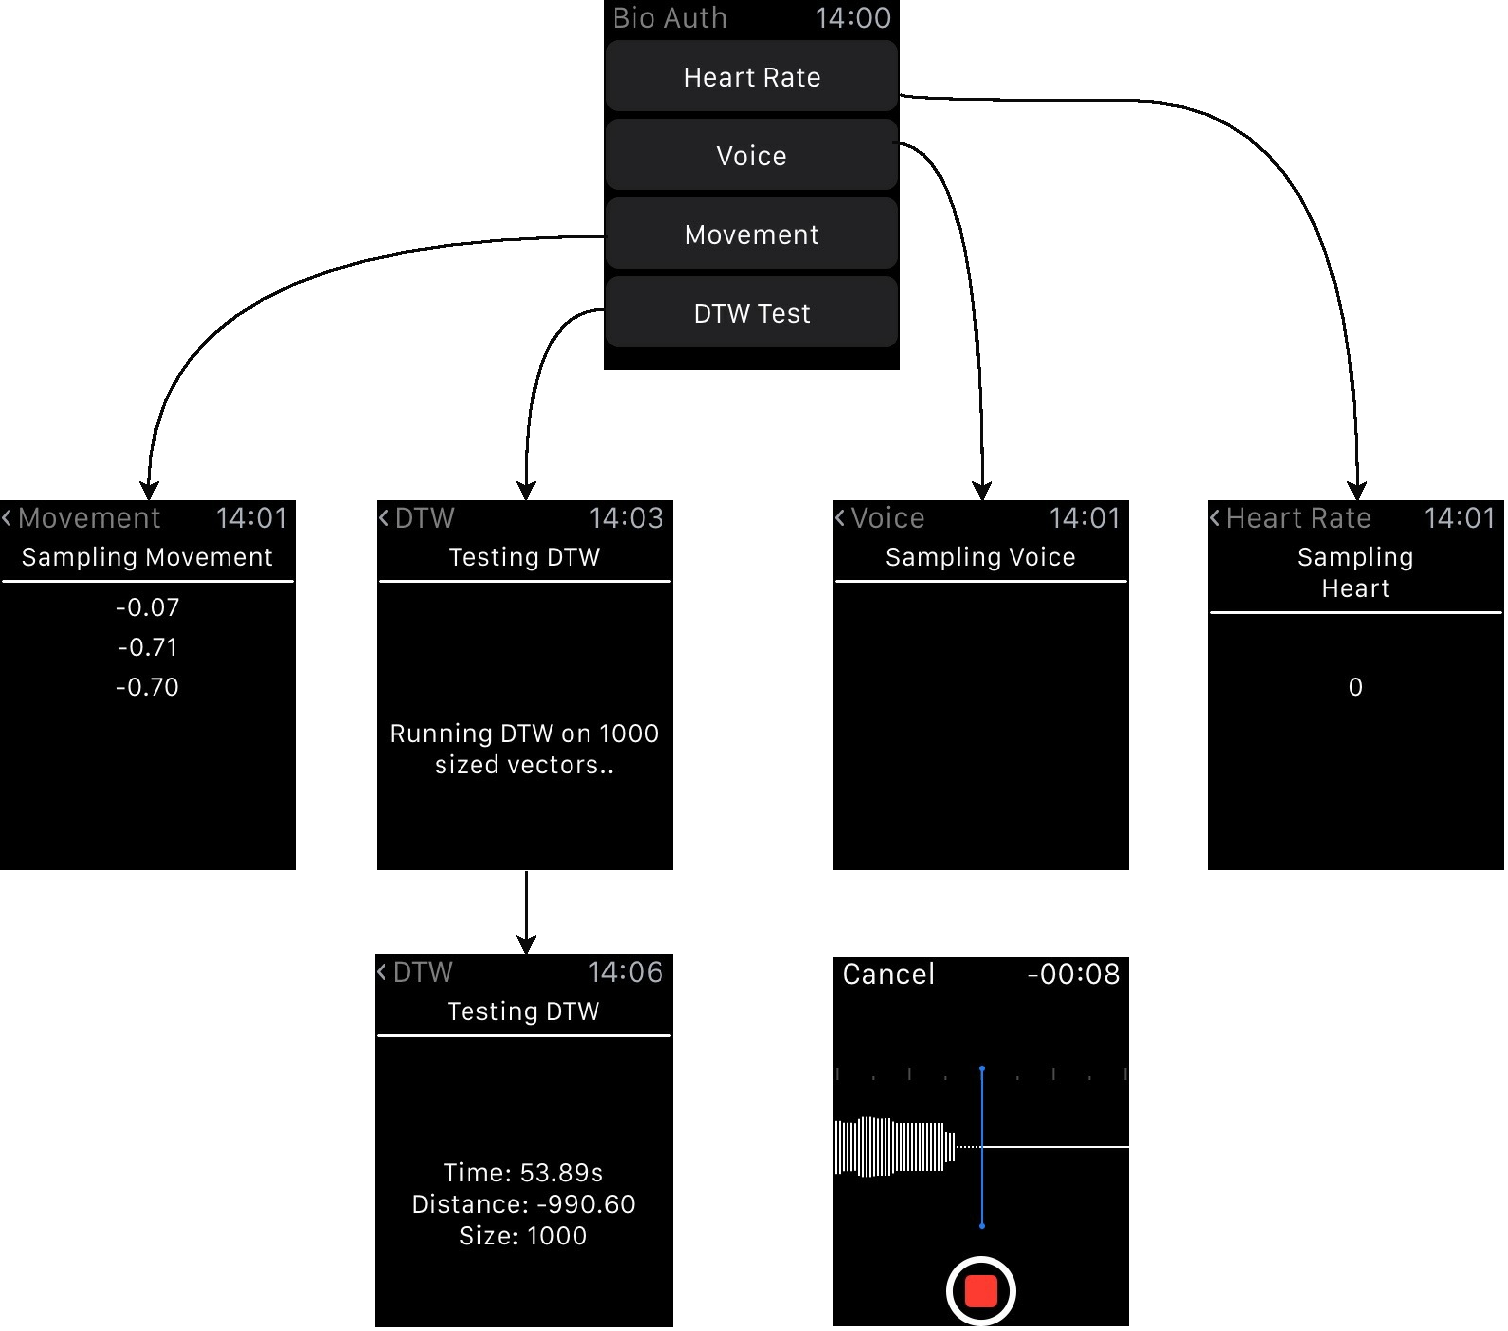
\includegraphics[width=0.8\textwidth]{../media/bioswp_ui.pdf}
\caption{Flow of the developed prototypes user interface. Start menu allows for
data extraction from the three sensors and to run DTW on arrays with 1000
    entries.}
\label{fig:ui}
\end{figure}

\begin{lstlisting}[label={lst:ui}, caption={Spawning of ViewControllers from the
main interface, passing contexts setting up the sampling.},basicstyle=\small]
@IBAction func movementButtonTapped() {
    let context = MovementInterfaceContext()
    context.instruction = "Sampling Movement"
    context.dataStorePath = "Movement_sample_\(NSTimeIntervalSince1970).data"
    context.sampleDuration = 10.0
    context.completionClosure = {() -> Void in print("Done")}
    self.pushControllerWithName("movementScene", context: context)
}

@IBAction func voiceButtonTapped() {
    let context = VoiceInterfaceContext()
    context.instruction = "Sampling Voice"
    context.dataStorePath = "Voice_sample_\(NSTimeIntervalSince1970).mp4"
    context.sampleDuration = 10.0
    context.completionClosure = {() -> Void in print("Done")}
    self.pushControllerWithName("voiceScene", context: context)
}

@IBAction func heartRateButtonTapped() {
    let context = HeartRateInterfaceContext()
    context.instruction = "Sampling Heart"
    context.dataStorePath = "HeartRate_sample_\(NSTimeIntervalSince1970).data"
    context.sampleDuration = 100.0
    context.completionClosure = {() -> Void in print("Done")}
    self.pushControllerWithName("heartRateScene", context: context)
}

@IBAction func dtwTestButtonTapped() {
    let context = DynamicTimeWarpInterfaceContext()
    context.instruction = "Testing DTW"
    context.testSampleSize = 1000
    self.pushControllerWithName("dtwScene", context: context)
}
\end{lstlisting}



\subsection{Microphone}
All functionality related to the microphone is handled by the microphone view,
which is controlled by the \texttt{VoiceInterfaceController}.
Here the recording interface is spawned to record the specified time. The
recording can be performed in a variety of qualities and formats, and is spawned
with the \texttt{WKInterfaceController} function
\texttt{presentAudioCon}-\texttt{trollerWithOutputURL}, see listing~\ref{lst:rec}. The format is
controlled by the file extension on the \texttt{NSURL} which the function saves
the recording to, and the quality is defined in the \texttt{preset}. The
different presets can be found in table~\ref{tbl:rec}.

\begin{lstlisting}[label={lst:rec}, caption={Spawning of the audio recording
    controller.},basicstyle=\small]
self.presentAudioRecorderControllerWithOutputURL(
    recFileUrl,
    preset: WKAudioRecorderPreset.WideBandSpeech,
    options: [
        WKAudioRecorderControllerOptionsMaximumDurationKey: 
            NSTimeInterval(duration)
    ],
    completion: { (didSave, error) -> Void in
        print("error: \(error)\n")
        if didSave {
            self.storeVoiceData(toFile, dataUrl: recFileUrl)
            self.popController()
        } else { self.popController() }
})
\end{lstlisting}

\begin{table}[!h]
\caption{Available audio recording presets, their sampling rate and bit rate.}
\label{tbl:rec}
\centering
\begin{tabular}{ |l|l|l|  }
\hline
\multicolumn{3}{|c|}{Audio Recorder Presets} \\
\hline
Preset             & Sample Rate & Format / Bit Rate\\
\hline
HighQualityAudio   & 44.1 kHz    & LPCM 705.6 kbps or AAC 96 kbps \\
WideBandSpeach     & 16 kHz      & LPCM 256 kbps or AAC 32 kbps \\
NarrowBandSpeach   & 8 kHz       & LPCM 128 kbps or AAC 24 kbps \\
\hline
\end{tabular}
\end{table}

\subsection{Accelerometer}
The accelerometer is accessed through the \texttt{CoreMotion} framework, which
provides a \texttt{CMMotionManager} one can attach sensor handlers to. Through
the manager it is possible to check if the accelerometer is available, set its 
update interval and attach a handler of the class
\texttt{CMAccelerometerHandler}. The handler receives updates of the defined
interval which, in the prototype, is saved to arrays for later storage. See
listing~\ref{lst:acc} for an example of how the accelerometer is accessed in the
prototype.
On the iPhone this is also the approach to retrieving data from the gyroscope,
but the watch returns \texttt{false} on the managers function
\texttt{gyroActive}. 

\begin{lstlisting}[label={lst:acc},caption={Usage of accelerometer in prototype.
The accelerometerHandler is attached to the motionManager in order to receive
updates on the set interval of 0.1.},basicstyle=\small]
motionManager.accelerometerUpdateInterval = 0.1
if motionManager.accelerometerAvailable {
    let accelerometerHandler:CMAccelerometerHandler = {
        (data: CMAccelerometerData?, error:NSError?) -> Void in
        if let data = data {
            self.xLabel.setText(String(format: "%.2f", data.acceleration.x))
            self.yLabel.setText(String(format: "%.2f", data.acceleration.y))
            self.zLabel.setText(String(format: "%.2f", data.acceleration.z))
            self.measuredDataX.append(data.acceleration.x)
            self.measuredDataY.append(data.acceleration.y)
            self.measuredDataZ.append(data.acceleration.z)
        }
        if let error = error {
            print(error.localizedDescription)
        }
        
    }
    if let duration = localContext?.sampleDuration {

        motionManager.startAccelerometerUpdatesToQueue(
            NSOperationQueue.currentQueue()!, 
            withHandler: accelerometerHandler)

        dispatch_after(dispatch_time(DISPATCH_TIME_NOW, 
                                     Int64(duration * Double(NSEC_PER_SEC))), 
                                     dispatch_get_main_queue()) {

            self.motionManager.stopAccelerometerUpdates()
            if let location = self.localContext?.dataStorePath {
                self.storeAccelerometerData(location,
                                            dataX: self.measuredDataX,
                                            dataY: self.measuredDataY,
                                            dataZ: self.measuredDataZ)
            }
        }
     }
}
\end{lstlisting}

\subsection{Heart Rate Sensor}
Heart rate data is accessed through the \texttt{HealthKit} framework. As
mentioned it is only possible to extract heart rate, and not the raw PPG data.
The heart rate sensor is started by starting a \texttt{HKWorkoutSession}, which
then records the health statistics, including the heart rate. The session is
started and stopped through the \texttt{HKHealthStore}, which also handles the
following queries for heart rate data. A query to the health store lets the
caller define sorting, limits to number of returned samples and predicates, such
as start and end time of the queried measurements, see listing~\ref{lst:queryhr}. 
The result from the query is injected into the \texttt{resultsHandler}, which in 
the prototype sends the data
to the phone.
In order to access the health data, one needs explicit permission by the owner 
of the device, which is requested on the watch and handled on the phone, through
the health stores function \texttt{requestToShareTypes}.
Beyond allowing for queries to the health store, after ended workout session, it
is also possible to receive a continuous stream of heart rate data, through a
\texttt{HKAnchoredObjectQuery}. This is utilized in the prototype to update the 
heart rate label on the watch, see listing~\ref{lst:streaminghr}.
A sample time of 100 seconds, results in approximately 20 samples of the
heart rate. The heart rate is not very useful for identification, but one could
hope that future versions will allow for raw data extraction.


\begin{lstlisting}[label={lst:queryhr},caption={Setting up a query for heart
rate samples. Including a time sorting descriptor, a date predicate and a
handler for the returned results.},basicstyle=\small]
let sortByTime = NSSortDescriptor(key: HKSampleSortIdentifierEndDate, 
                                  ascending: false)
let datePredicate = 
    HKQuery.predicateForSamplesWithStartDate(startDate, 
                                             endDate: endDate, 
                                             options: HKQueryOptions.None)
let query = 
    HKSampleQuery(
      sampleType: heartRateType,
      predicate: datePredicate,
      limit: 1000,
      sortDescriptors: [sortByTime],
      resultsHandler: {(query, results, error) in
        guard let results = results else { return }
        for sample in results {
            let quantity = (sample as! HKQuantitySample).quantity
            let heartRateUnit = HKUnit(fromString: "count/min")
            heartRateArray.append(quantity.doubleValueForUnit(heartRateUnit))
        }
        ...
    })
self.healthStore.executeQuery(query)
\end{lstlisting}

\begin{lstlisting}[label={lst:streaminghr},caption={Setting up a streaming heart
rate query for continuous handling of samples generated by the heart rate
sensor.},basicstyle=\small]
func getHeartRateStreamingQuery(workoutStartDate: NSDate) -> HKQuery? {
    guard let quantityType = HKObjectType.quantityTypeForIdentifier(
                                HKQuantityTypeIdentifierHeartRate) 
                             else { return nil }
    let heartRateQuery = 
        HKAnchoredObjectQuery(
            type: quantityType,
            predicate: nil,
            anchor: anchor,
            limit: Int(HKObjectQueryNoLimit))
            {(query, sampleObjs, deletedObjs, newAnchor, error) -> Void in
                  guard let newAnchor = newAnchor else { return }
                  self.anchor = newAnchor }

    heartRateQuery.updateHandler = 
        {(query, sampleObjs, deletedObjs, newAnchor, error) -> Void in
            self.anchor = newAnchor!
            self.updateHeartRate(sampleObjs)}
    return heartRateQuery
}
\end{lstlisting}

\subsection{Dynamic Time Warp}
The implementation of DTW is only included to showcase the computational power of
the \textit{Apple Watch}, and to evaluate if it is viable to run such a rather
heavy algorithm on the watch.
The DTW algorithm has beenMotion Sensors implemented in the class
\texttt{DynamicTimeWarper}. The class only has a single function,
    \texttt{distance}, which takes to arrays of doubles, and returns the
    calculated distance between the two. The algorithm is run by the
    \texttt{DynamicTimeWarpInterfaceController}, which tracks how long time the
    algorithm takes to execute the algorithm, on arrays filled with random data. 
As seen in table~\ref{tbl:dtw} the complexity is as expected $O(n^2)$.
This makes it viable to run smaller sets with this algorithm, and other distance
measuring algorithms could probably also run on the device.
Another approach could be to execute the algorithm on the connected iPhone,
which would result in a significant performance boost, due to the more powerful
hardware. This would allow for more complex algorithms on largers sets of data.


\begin{lstlisting}[label={lst:dtw},caption={Testing of the implemented DTW
    algorithm, within the DynamicTimeWarpInterfaceController},basicstyle=\small]
dispatch_async(queue) {
    let dtw = DynamicTimeWarper()
    let testArr1 = 
        (0...localContext.testSampleSize!).map {_ in drand48()}
    let testArr2 = 
        (0...localContext.testSampleSize!).map {_ in drand48()}
    let distance = 
        String(format: "%.2f", dtw.distance(testArr1, target: testArr2))
    let deltaTime = 
        String(format: "%.2f", abs(self.dtwStart!.timeIntervalSinceNow))
    self.resultLabel.setText("Time: \(deltaTime)s\n
                              Distance: \(distance)\n
                              Size: \(localContext.testSampleSize!)")
}
\end{lstlisting}

\begin{table}[!h]
\caption{Measured time it takes to run DTW on different sized arrays.}
\label{tbl:rec}
\centering
\begin{tabular}{ |c|c|  }
\hline
Array Size  & Time in seconds\\
\hline
100    &        \\
250    &        \\
500    &        \\
1000   & 53.89  \\
\hline
\end{tabular}
\end{table}

\subsection{Data transfer and storage}
In order to extract the data from the watch, it is sent to the iPhone in a
message. The iPhone ensures that the data is stored in the \textit{Documents}
directory, so the data easily can be extracted. This process happens after each
sampling from a sensor. The library \texttt{WatchConnectivity} handles transfers
of messages and files through sessions. The session is initiated both on the
watch, and on the phone. An example of usage on the watch can be found in 
listing~\ref{lst:wcsessionsend} and the receiving example can be found in 
listing~\ref{lst:wcsessionreceive}.
After succesful transfer, the samples can be downloaded from the phone through
iTunes.
This approach could also be used if processing of the measured data should be
performed on the phone instead.

\begin{lstlisting}[label={lst:wcsessionsend},caption={Send heart rate data to the
phone from the watch.},basicstyle=\small]
self.session = WCSession.defaultSession()
self.session!.sendMessage(
    ["heartRateArray": heartRateArray, "location": location],
    replyHandler: {(response) -> Void in
        print("Succesful heart-rate msg to phone")
    },
    errorHandler: {(error) -> Void in
        print("Unsuccesful heart-rate msg to phone")
    })
\end{lstlisting}

\begin{lstlisting}[label={lst:wcsessionreceive},caption={Receiving heart rate
data on phone, and storing it to the Documents folder.},basicstyle=\small]
func session(session: WCSession, 
             didReceiveMessage message: [String : AnyObject], 
             replyHandler: ([String : AnyObject]) -> Void) {
...
    let documentsDir = try NSFileManager.defaultManager()
                           .URLForDirectory(.DocumentDirectory, 
                                            inDomain: .UserDomainMask,
                                            appropriateForURL: nil, 
                                            create: true)
    guard let location = message["location"] as? String else {return}
    if let heartRateArray = message["heartRateArray"] as? Array<Double> {
        if let pathUrl = NSURL(string: location, relativeToURL: documentsDir) {
            try heartRateArray.description
                              .writeToURL(pathUrl, 
                                          atomically: true, 
                                          encoding: NSASCIIStringEncoding)
            replyHandler([:])
        }
    }
...
\end{lstlisting}
